% Updated in May 2014 by Hideo Saito
% Updated in March 2012 by Yasuyuki Matsushita
% Updated in April 2002 by Antje Endemann, ...., and in March 2010 by Reinhard Klette
% Based on CVPR 07 and LNCS style, with modifications by DAF, AZ and elle 2008, AA 2010, ACCV 2010

\documentclass[runningheads]{llncs}
\usepackage{graphicx}
\usepackage{amsmath,amssymb} % define this before the line numbering.
\usepackage{ruler}
\usepackage{color}
\usepackage{cite}
\usepackage{pifont}

%===========================================================
% Commands
\newcommand{\B}[1]{{\color{red}[Bernard: #1]}}
\newcommand{\JC}[1]{{\color{red}[JC: #1]}}

%===========================================================
\begin{document}
\pagestyle{headings}
\mainmatter

\def\ACCV14SubNumber{165}  % Insert your submission number here

%===========================================================
\title{Surrounding cues for human action recognition} % Replace with your title
\titlerunning{ACCV-14 submission ID \ACCV14SubNumber}
\authorrunning{ACCV-14 submission ID \ACCV14SubNumber}

\author{Anonymous ACCV 2014 submission}
\institute{Paper ID \ACCV14SubNumber}

\maketitle

%===========================================================
\begin{abstract}
This paper describes a framework for recognizing human actions in videos by incorporating a new set of visual cues that represent the \emph{context} of the action. We develop a weak foreground-background segmentation approach in order to robustly extract not only foreground features that are focused on the actors, but also global camera motion and contextual scene information. Using dense point trajectories, our approach separates and describes the foreground motion from the background, represents the appearance of the extracted static background, and encodes the global camera motion that interestingly is shown to be discriminative for certain action classes. Our experiments on four challenging benchmarks (HMDB51, Hollywood2, Olympic Sports, UCF50) show that our contextual features enable a significant performance improvement over state-of-the-art algorithms.

\end{abstract}

%===========================================================
\section{Introduction}
\label{introduction}
%\section{Preliminaries}
\label{preliminaries}
\subsection{Camera compensation using Fundamental Matrix}
\subsection{Foreground/Background trajectories}

\section{Proposed Methodology} \label{scene}

\begin{figure*}[t!]
\begin{center}
%\fbox{\rule{0pt}{3in} \rule{0.9\linewidth}{0pt}}
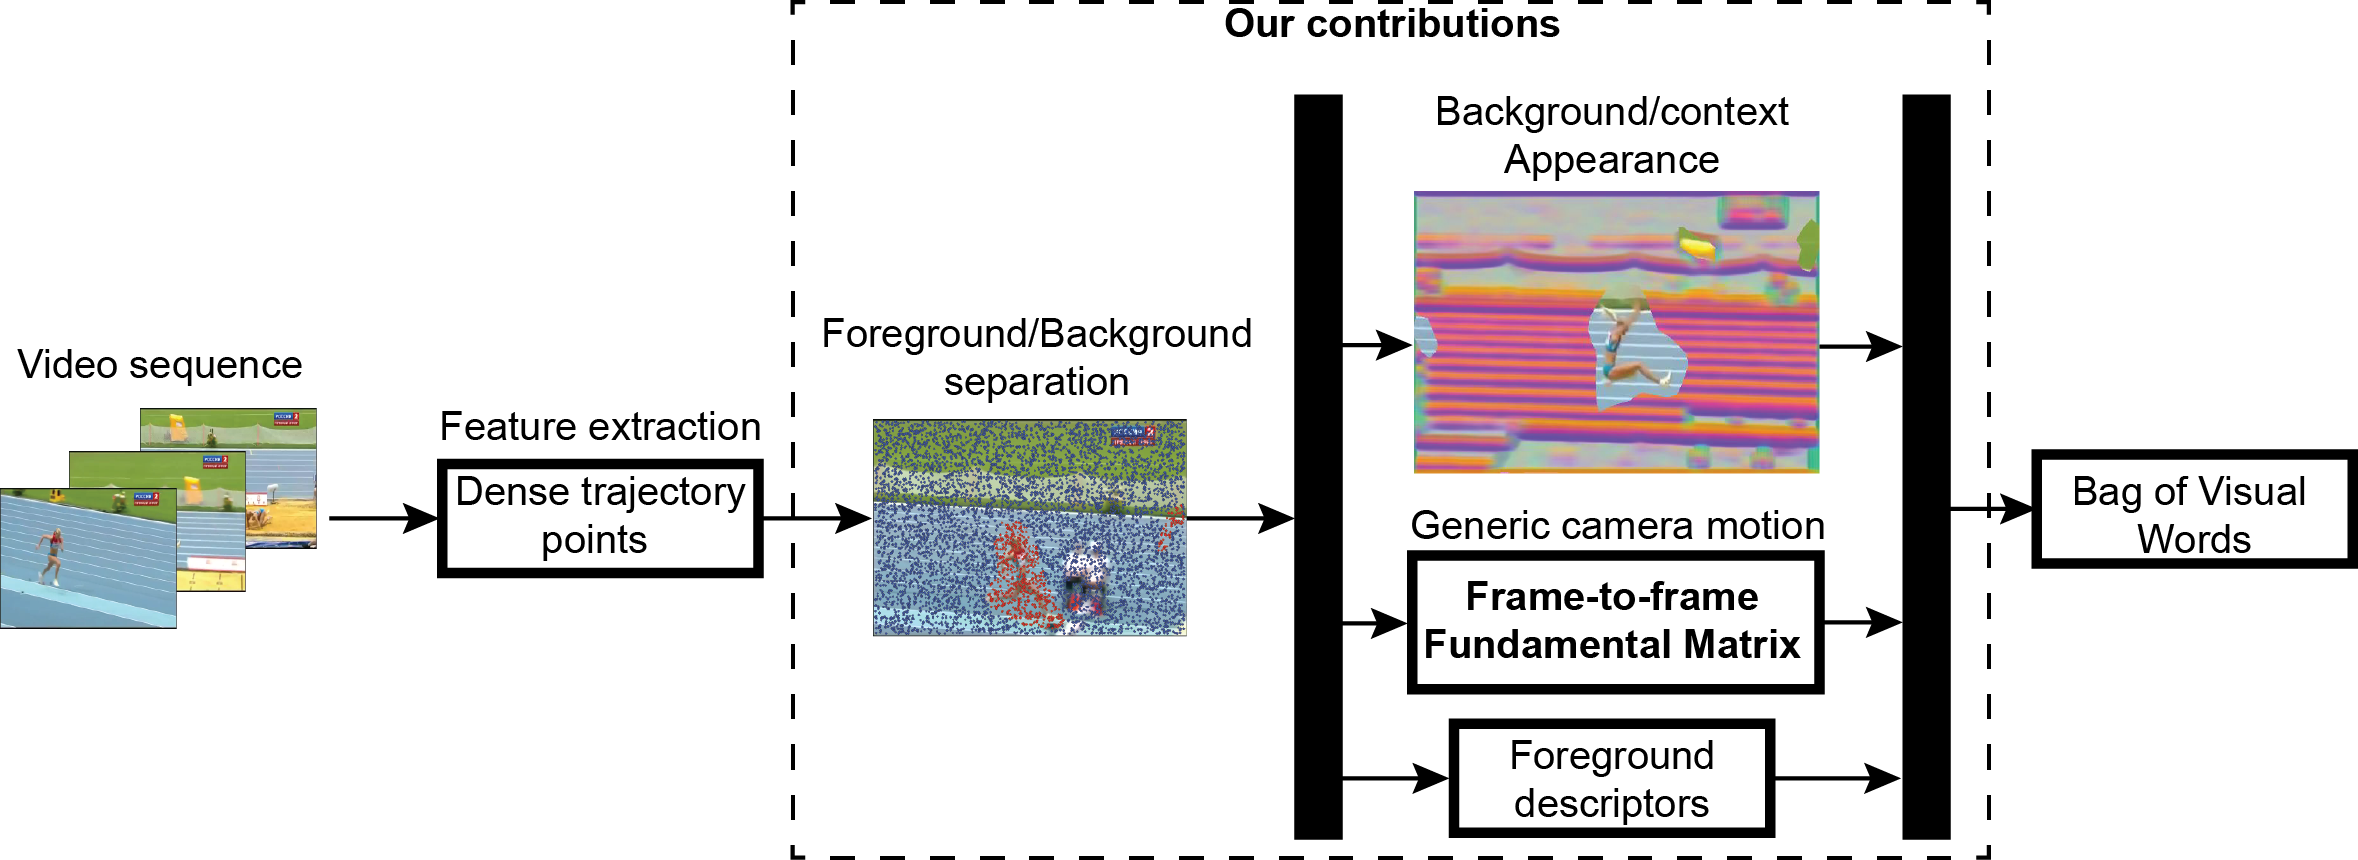
\includegraphics[width=0.98\linewidth]{fig/pipeline.png}
\end{center}
\caption{Given a video sequence, a set of dense points trajectories are extracted. Then, a Fundamental Matrix is used to apply a camera compensation and to separate foreground and background trajectories. Each type of trajectories are encoded by different type of descriptors. Specifically, a low level global motion is used to generally describe the camera motion. Moreover, context appearance is explicitly computed on background trajectories. Traditional foreground descriptors (\eg MBH, HOF, HOG and trajectory shape) are also aggregated in actions description. Finally, this set of descriptors are encoded separately using the BoF framework.}
\label{fig:pipeline}
\end{figure*}

This section gives a detailed description of our proposed approach for action recognition in video. The methodology in this paper follows the conventional action recognition pipeline. Given a set of labelled videos, a set of features is extracted from each video, represented using visual descriptors, and combined into a single video descriptor, which is used to train a multi-class classifier for recognition.

%\B{It will be easier to have a pipeline image that shows the different stages of processing: (1) extract dense improved trajectories, (2) foreground/background trajectory separation, (3) compute descriptors for the foreground (BoF on MBH, HOF, etc for each trajectory), the camera motion (BoF on frame-to-frame estimated fundamental matrices), and the context (BoF on the background appearance).}

In this paper, we use dense point trajectories (short tracks of a densely sampled set of pixels in a video \cite{wang2013}) as our primitive features. By estimating frame-to-frame camera motion (fundamental matrix), we separate foreground trajectories corresponding to the action from background ones. Each type of trajectory is represented using a different descriptor. Foreground trajectories are represented using conventional visual properties (e.g. MBH, HOF, HOG, and trajectory shape), while the background appearance is described using SIFT. Foreground and background trajectories are then encoded separately using the BoF framework as illustrated in Figure \ref{fig:pipeline}. Unlike other action recognition methods, we not only use the frame-to-frame camera motion to separate foreground from background, but we also use it to \emph{describe} a video. This is done by encoding all frame-to-frame fundamental matrices in a video using the BoF framework. We use all three descriptors (foreground, background/context, and camera motion) to train a multi-class classifier for recognition. In this paper, we argue and show that combining a foreground-only description \cite{wang2013} with additional cues (background/context and camera motion) provides a richer and more discriminative description of actions.

%\B{\st{Since camera motion is used in the foreground-background separation part too, I recommend we move the the camera motion subsection to be first, then the  separation subsection, then the context/background subsection}}


%describes our methodology for capturing background information or \textit{contextual features}. We present a novel approach for including description of background trajectories. We argue that combining a pure foreground description \cite{wang2013} with additional surrounding cues have a significant contribution to action description. To obtain these background trajectories, we perform a weak foreground-background separation based on the trajectory displacement. Then, we explicitly model the global motion in the video and the context appearance using those background feature points.

\subsection{Generic Camera Motion}
Since videos are normally filmed with the intention of maintaining the subject within the image frame, there exists a relationship between the estimated camera motion and the underlying action. In this paper, we argue and show that this relationship can be a useful cue for discriminating certain action classes. As observed in the three top rows of Figure \ref{fig:camMotion_example}, there is a correlation between how camera moves and the subject, \eg in the second row, the \textit{cameraman} operates a till down in order to register the movement of the diver. Here, we do not claim that this cue is significant for all types of actions, since very similar camera motion can be shared among classes. Also, several actions not involves subjects translations, as noticed in Figure \ref{fig:camMotion_example} (\textbf{last two rows}). Instead of using a homography to encode camera motion, we estimate the more general fundamental matrix for each pair of frames in a video using the well-known 8-point algorithm \cite{eightpoint97}. As mentioned earlier, a homography is suitable to describe camera motion when the camera is not translating or when the background is planar; however, it is not applicable in more complex or cluttered scenes.

In our experiments, we calculate \textbf{camera motion descriptors} as follows. After estimating all pairwise fundamental matrices using RANSAC, we encode the camera motion of a video using the BoF framework. We call this descriptor CamMotion and it is complementary to other visual descriptors of the video. Unlike most existing work, we embrace camera motion and employ a low-level feature to capture this global motion in the video.



\subsection{Foreground-Background Separation}
We now consider a camera compensation using our global motion model introduced in section \ref{subsec:cam_motion}. Exploiting the well performance of this compensation, we can easily separate trajectory points associated with the background, which tend to present a small displacement over the length of the trajectory. Taking advantage of this, we threshold trajectory displacement to obtain a foreground-background separation. The trajectory displacement is computed as follow:

%In order to recover foreground action only information, we need to separate the extracted dense trajectories into foreground or background. Some information related to the actor are included on the Improved Trajectories approach. It results beneficial when capturing the spatio-temporal appearance of human actions. However, we claim that modeling contextual information needs to be performed on background feature points. \B{Fabian, the previous three sentences need to be rephrased and expanded for clarity. I didnt quite understand what you meant here.} We apply a simple strategy to weakly label trajectory features. We compute trajectories as described in \cite{wang2013}, but also compute the sum of the Frobenius norm for the displacement vector as follows:

\begin{equation}
D = \sum _{j=t}^{t+L-1}\left ( (x_{t+1}-x_t)^2, (y_{t+1}-y_t)^2 \right ).
\end{equation}

Trajectory points are associated with the background if $D<=\alpha$. Otherwise, those trajectory points are labeled as foreground. Empirically, we set this threshold value to $\alpha=3$ pixels.

Figure \ref{fig:approach} shows an example of our foreground-background separation in a video associated with the action \textit{long jump}. Here, foreground and background trajectories are color-coded in red and blue respectively. Clearly, the foreground trajectories correspond to the underlying action itself, while background trajectories correspond to \emph{static} background pixels undergoing camera motion only. Our proposed separation will allow each type of trajectory (foreground and background) to be represented independently and thus more reliably than other methods that encode context information using features from the entire frame \cite{marszalek2009}.

In practice, we calculate \textbf{foreground descriptors} that consist of Trajectory Shape, HOG, HOF, and MBH computed over dense trajectories using an implementation modified from \cite{wang2013}. In the following section, we detail how background appearance is encoded.


\begin{figure*}[t!]
\begin{center}
%\fbox{\rule{0pt}{3in} \rule{0.9\linewidth}{0pt}}
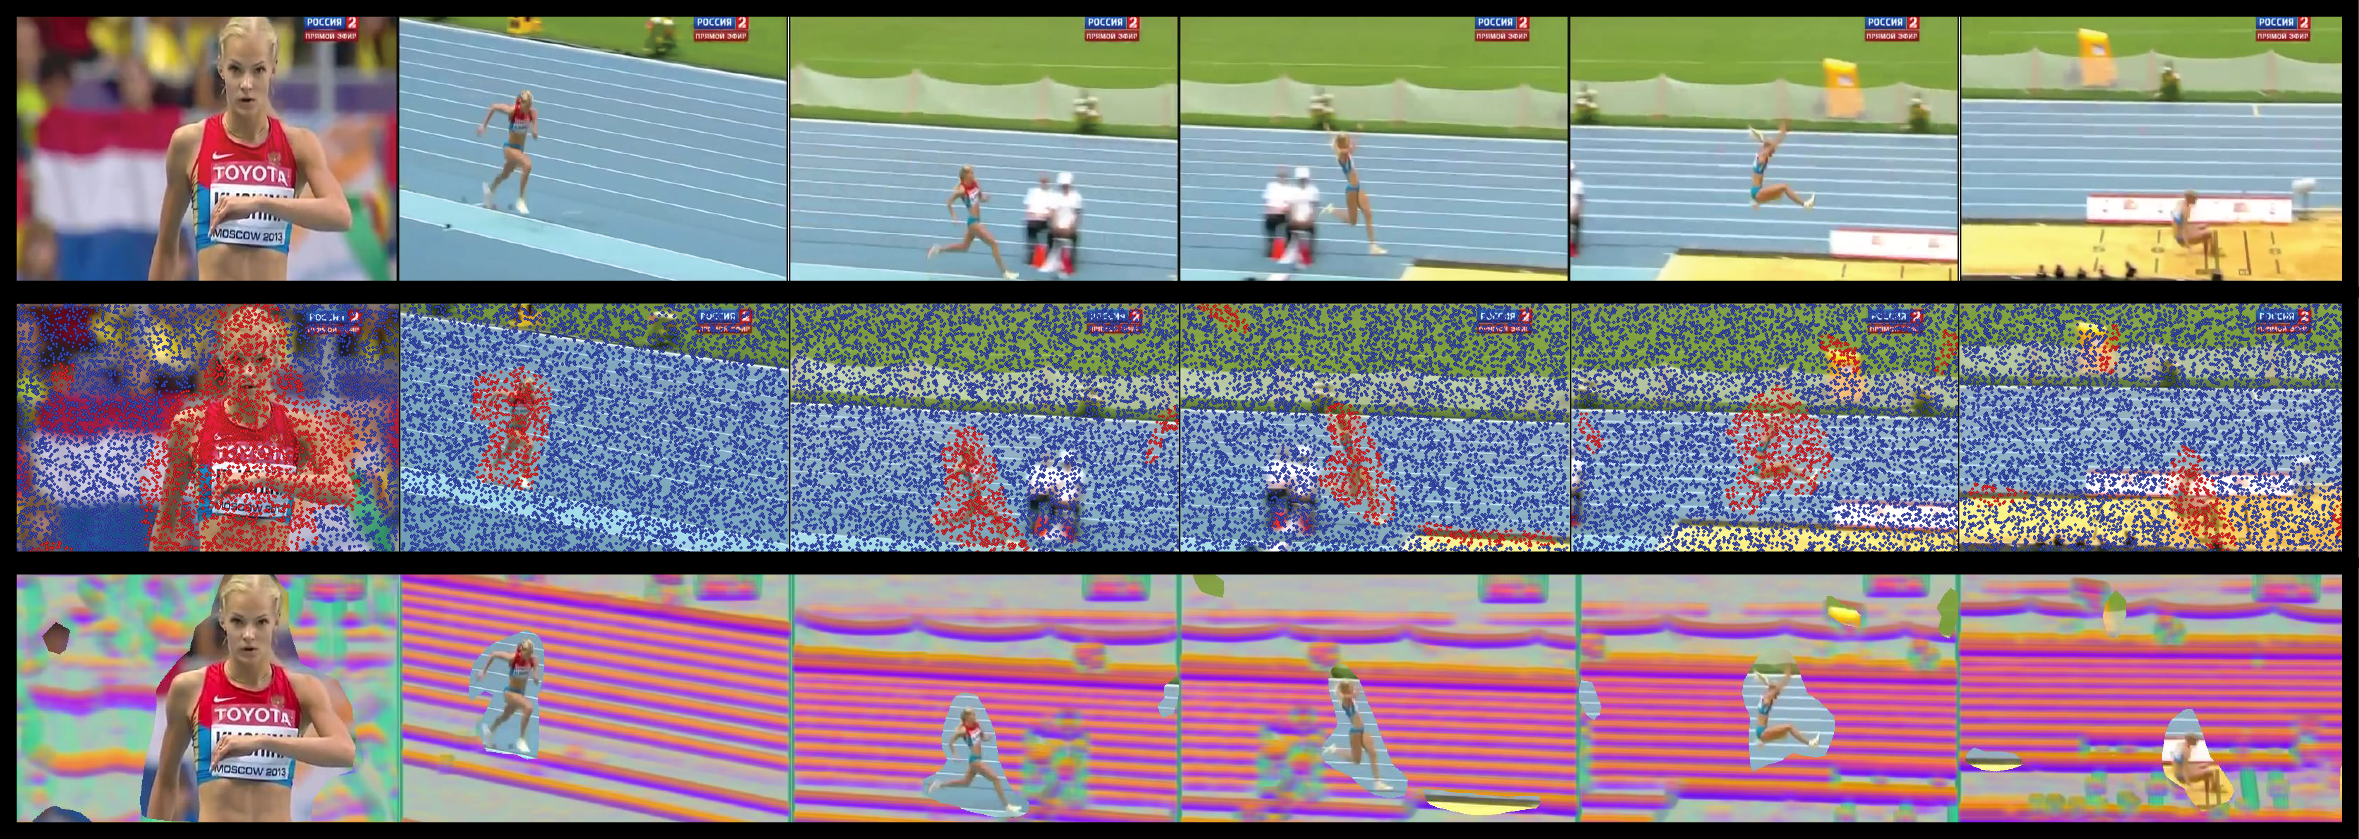
\includegraphics[width=0.98\linewidth]{fig/approach.png}
\end{center}
\caption{Overview of our method. \textbf{Top}. Frame sequence sampled from a long jump video. Note that the video contains a translation movement following the subject. \textbf{Middle}. Camera compensation allows to perform a background-foreground segmentation. Noticeably, foreground feature points are mostly related with the subject. \textbf{Bottom}. Illustration of captured information by SIFT. In order to achieve a meaningful illustration, descriptor dimensionality is reduced to 3 dimensions and output within a color code image. As illustrated, contextual appearance is captured only from pixels related with the scenario \ie avoiding pixels related with the subject with execute the action.}
\label{fig:approach}
\end{figure*}


\subsection{Background/Context Appearance}
Human actions could be recognized by a set of cues. Beyond local motion and appearance properties of an action, the context in which an action is performed is a critical component to recognize actions. For example, a 'springboard' action can only be executed if there is a pool, which has distinctive appearance properties. This motivates us to encode the visual appearance of the static scene. Background/context appearance is encoded using SIFT descriptors \cite{lowe2004} around trajectory points associated with the background. We detect SIFT keypoints in a dense manner and then filter out those that fall within the union of foreground trajectories. Context appearance focuses more on the scenario itself, as observed in Figure \ref{fig:approach}. Additionally, in Figure \ref{fig:sift_example} is noticed how context appearance can be used to aggregate meaningful information about the action. For example, all presented thumbnails for the action rowing contains a shared landmark which can be exploited modeling the appearance of background points.  Unlike other methods that scene encode context holistically in a video \cite{marszalek2009}, separating the background/context from the foreground produces a more reliable and robust context descriptor.

\begin{figure*}[t!]
\begin{center}
%\fbox{\rule{0pt}{3in} \rule{0.9\linewidth}{0pt}}
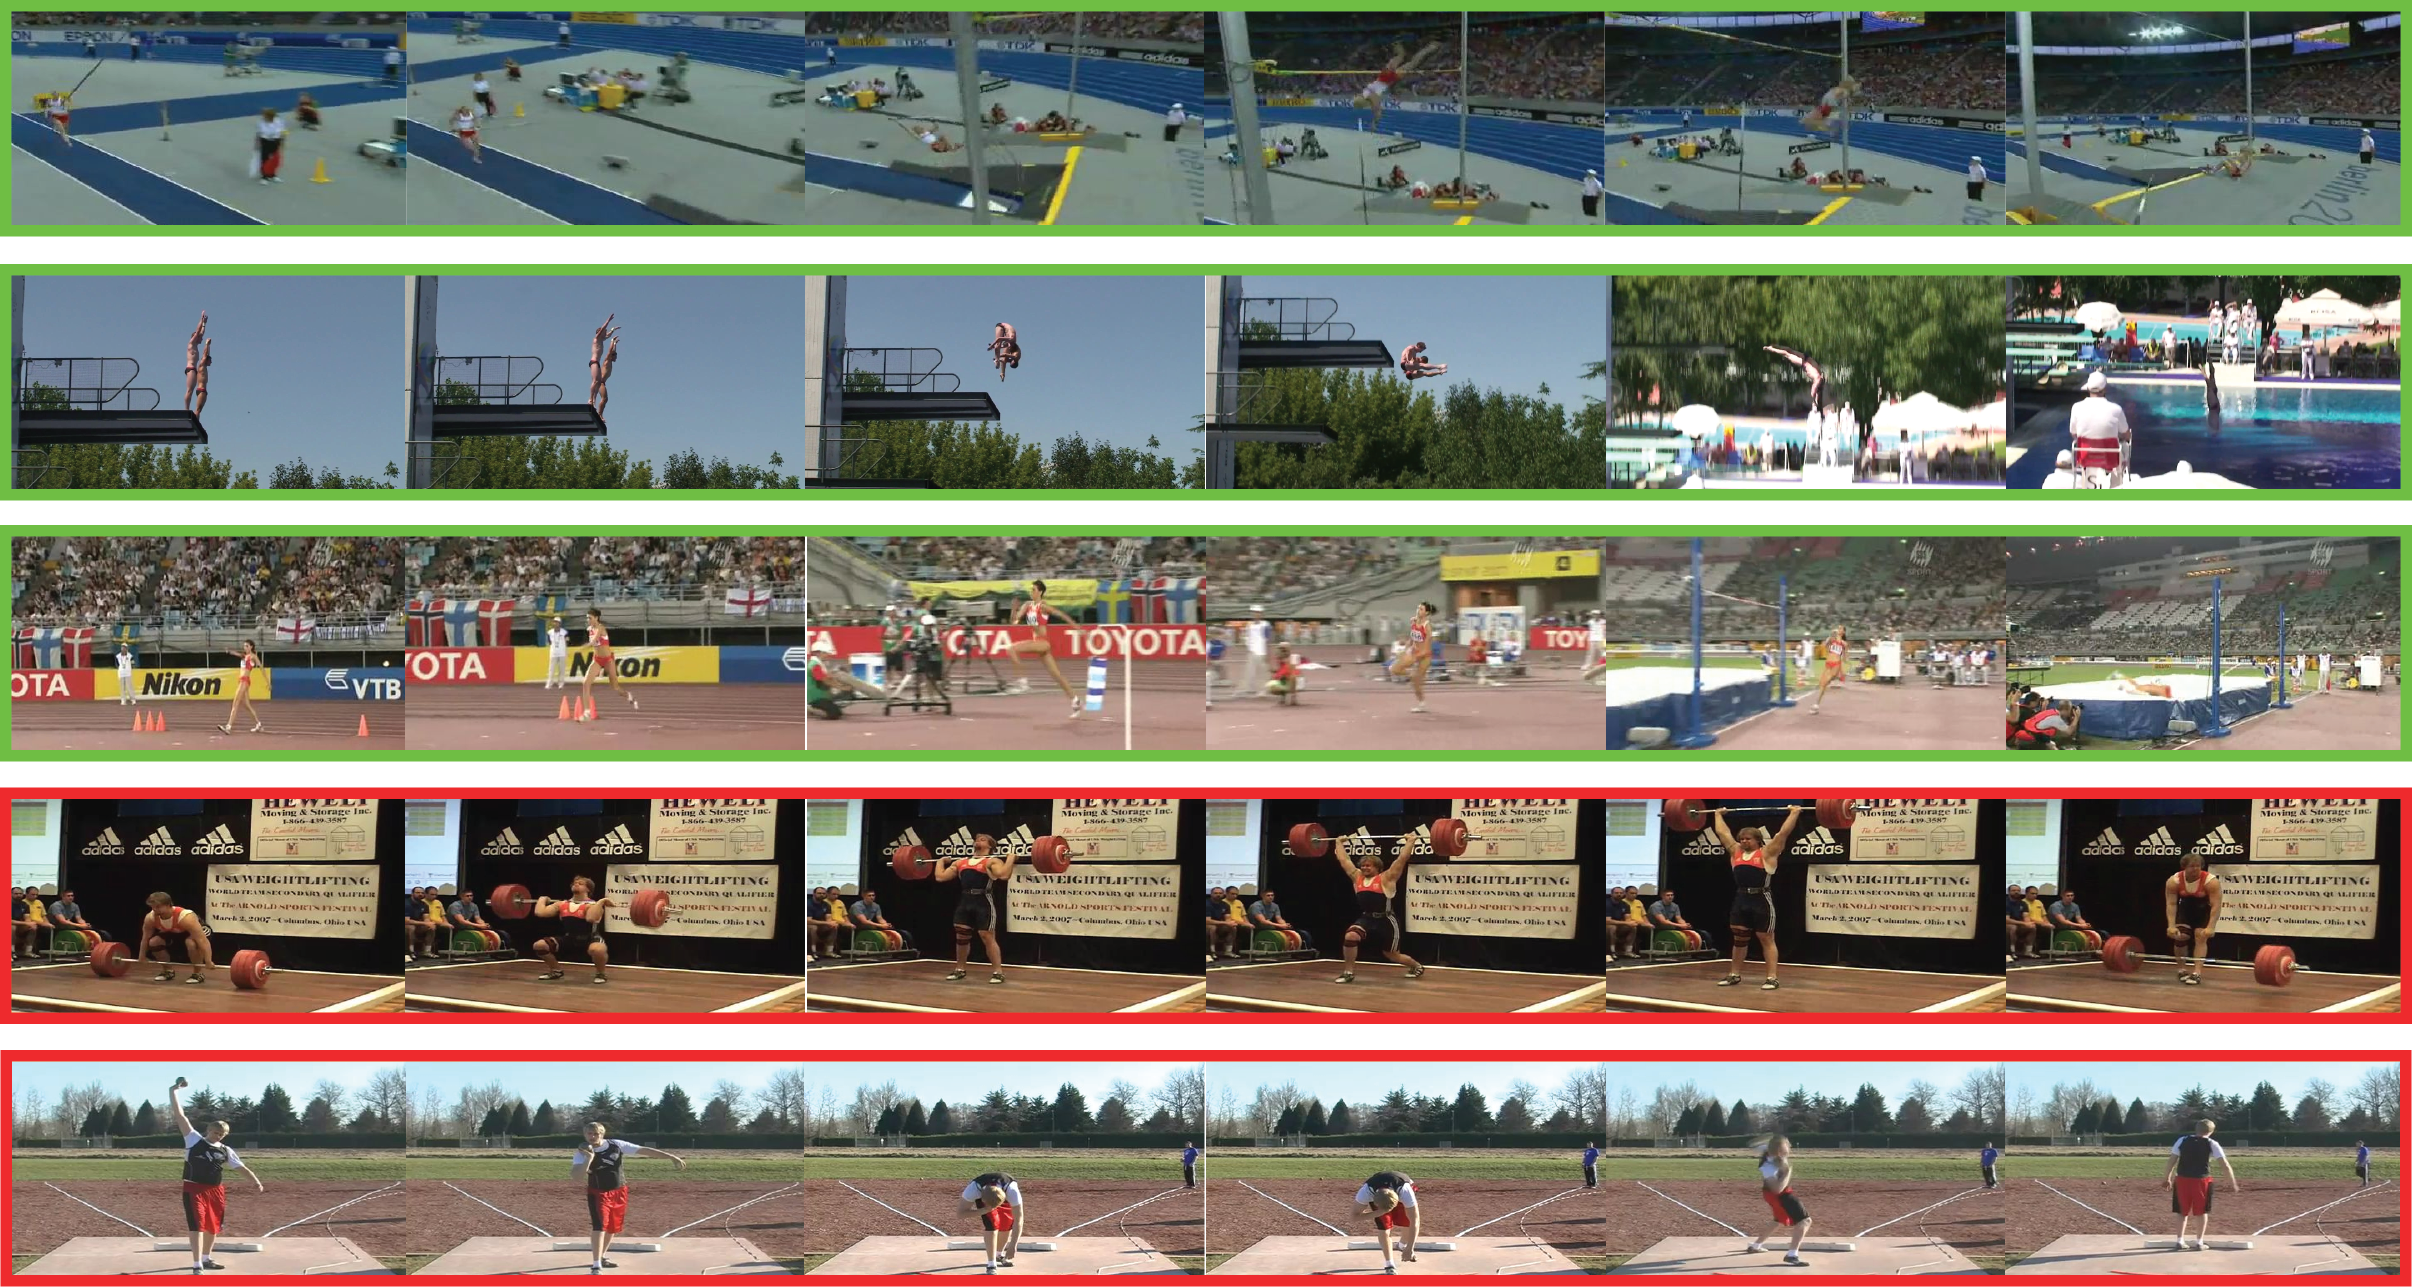
\includegraphics[width=0.98\linewidth]{fig/camMotion.png}
\end{center}
\caption{A generic camera motion descriptor can be a useful cue for discriminating specific action categories. As illustrated, the first three rows contains a characteristic correlation between how camera moves and the associated action. Unfortunately, this type of cue its not significant for all type of actions as shown in the last two rows where camera not move at all.}
\label{fig:camMotion_example}
\end{figure*}

\begin{figure*}[t!]
\begin{center}
%\fbox{\rule{0pt}{3in} \rule{0.9\linewidth}{0pt}}
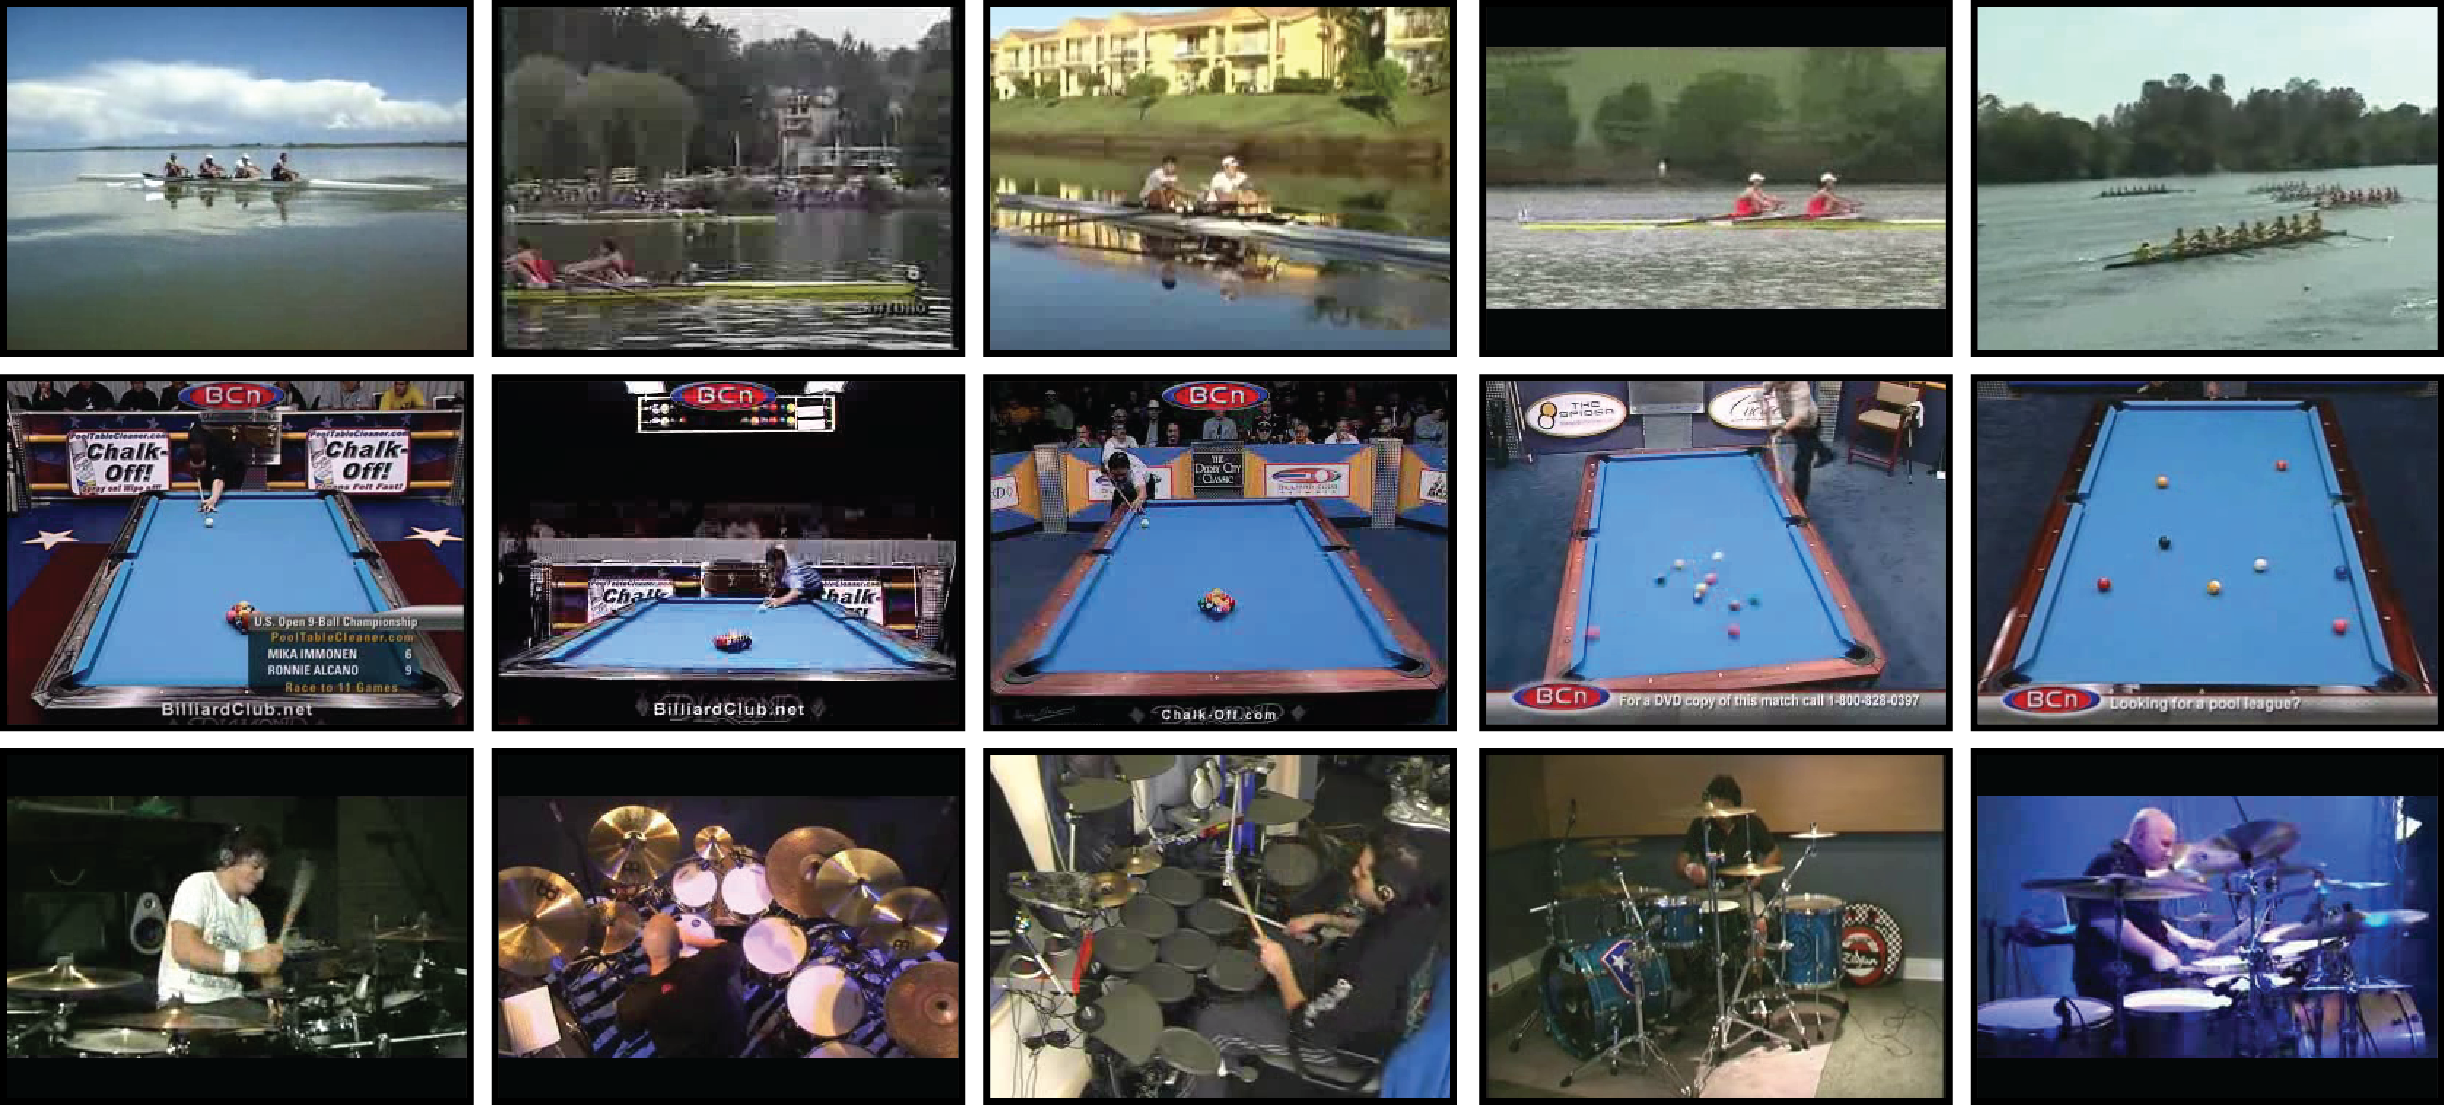
\includegraphics[width=0.98\linewidth]{fig/sift.png}
\end{center}
\caption{Each row presents five different thumbnails taken from different videos of UCF50 dataset. \textbf{Top} row corresponds to rowing's examples. As observed all thumbnails share distinct background appearance \ie in all water is present and also in the majority there is a common landmark. In the \textbf{Middle} row, different billiard examples are depicted. Billard table and also the indoor naturalness of the action, enables context appearance to capture critical information about the action. Finally, \textbf{Bottom} row exposes examples from the drumming category. As noticed, all of the examples share a lot of visual cues that mostly are avoided if only foreground features are used.}
\label{fig:sift_example}
\end{figure*}



\subsection{Implementation details}

\textbf{Codebook generation}. We generate the visual codebook in two different ways: (a) using \textbf{\textit{k}-means}, where we cluster the visual space, or, (b) using a \textbf{Gaussian Mixture Model (GMM)}, which captures a probability distribution over feature space. In both cases, a codebook is computed for each descriptor separately. Because of trajectory points methodologies produces a large amount of features resulting in intractable codebook computations, it is necessary to sub-sample the features extracted in the training examples for the purpose of codebook generation. In order to establish a trade-off between computation cost and recognition performance, we study the effect of the number of sampled features for computing a visual codebook, as observed in Figure \ref{fig:feature_sampling}. This experiment includes results in two different datasets using \textit{k}-means to form the visual dictionary. Additionally, we employ a spatial clustering sampling which shows a better performance compared to the uniform sampling. Mentioned spatial clustering finds K centers using \textit{k}-means over all features in a video. Then, the nearest trajectories on that centers are selected as the features to describe the video. In the following, we employ approximately 5 millions of feature points (~8GB RAM required per descriptor) sampled with a spatial clustering to form visual codebooks.\\\\
\textbf{Feature encoding} is performed under two different methodologies: (a) following the traditional histogram quantization (VQ), or, (b) applying the recently introduced Fisher vectors \cite{perronnin2010}. Different types of \textbf{Normalization} are performed to make feature vectors more robust: (a) \textit{l2} normalization (L2) \cite{perronnin2010}, (b) power normalization (PW) \cite{perronnin2010} and (c) intra-normalization (IN) \cite{xwang2013}. \\\\
\textbf{Framework representation}. We adopt two majors frameworks for action recognition. One of them follows the Bag of Features (BoF) paradigm, using \textit{k}-means for computing visual codebook, encoding features using VQ and L2 normalization, and finally learning action models with a non-linear SVM with $\chi^2$ kernel within a multichannel approach (MCSVM) as in \cite{zhang2007}:
\begin{equation}
K(x_i,x_j)= \exp(-\sum_c {\frac{1}{2\Omega_c} D_c(x_i,x_j)}),
\label{eq:multichannel}
\end{equation}
where $D_c(x_i,x_j)$ is the $\chi^2$ distance for channel $c$, and $\Omega_c$ is the average channel distance. Moreover, we implement a more robust framework (Fisher vectors) learning a codebook using a GMM. Consequently, we encode the feature vectors using the Fisher vectors. In this case, we apply three normalization strategies, L2, PW and IN as proposed in \cite{xwang2013}. Finally, normalized channels are concatenated and action models are learned within a linear SVM (LSVM). Described approaches are summarized in Table \ref{tab:frameworks}.

%%%%%%%%%%%%%%%%% Figure: Effect of sampling %%%%%%%%%%%%%%%%%%%
\begin{figure*}[t!]
\begin{center}
%\fbox{\rule{0pt}{1.2in} \rule{0.9\linewidth}{0pt}}
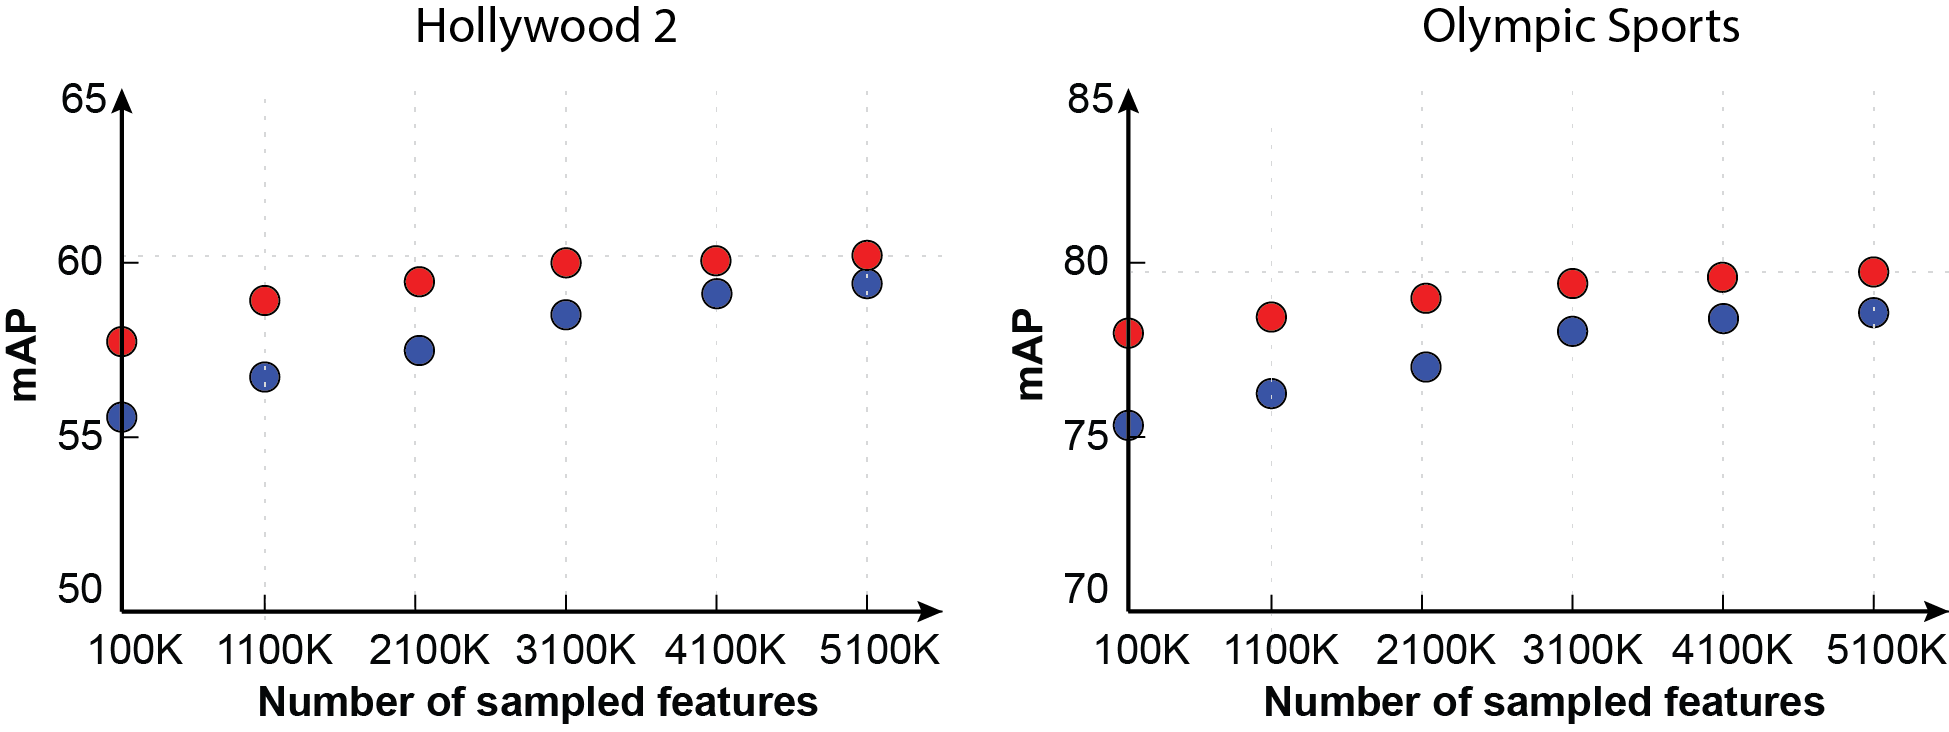
\includegraphics[width=0.98\linewidth]{fig/sampling.png}
\end{center}
\caption{Effect of feature sub-sampling when generating codebook.}
\label{fig:feature_sampling}
\end{figure*}
%%%%%%%%%%%%%%%%%%%%%%%%%%%%%%%%%%%%%%%%%%%%%%%%%%%%%%%%%%%%%%%%


%%%%%%%%%%%%%%% Table: Frameworks comparison %%%%%%%%%%%%%%%%%%%
\begin{table*}[h!]
\caption{Comparison of adopted frameworks for action recognition.}
\begin{center}
{
\begin{tabular}{ l| c c c c c }
\hline
Representation $\downarrow$ & Codebook & Encoding & Normalization & Classifier \\
\hline
Bag of Features & \textit{k}-means & VQ & L2 & MCSVM \\
Fisher vectors & GMM & Fisher vectors & L2+PW+IN & LSVM \\
\hline
\end{tabular}
}
\end{center}
\label{tab:frameworks}
\end{table*}
%%%%%%%%%%%%%%%%%%%%%%%%%%%%%%%%%%%%%%%%%%%%%%%%%%%%%%%%%%%%%%%%



\section{Experimental results}
\label{results}
\subsection{Datasets and evaluation protocol}
\label{subsec:datasets}
We use four public datasets \cite{kuehne2011, marszalek2009, niebles2010, reddy2013} and their corresponding evaluation protocols. In this section we briefly describe each dataset.

\textbf{HMDB51} \cite{kuehne2011} includes a large collection of human activities categorized on 51 classes. It collects 6766 videos from different media resources \ie digitized movies, public databases and user generated web video data. Due to a large amount of videos contains undesired camera motions, the authors provide a stabilized version of the dataset. However, since we look at the camera motion as an informative cue, non-stabilized version of the dataset is used. For evaluating performance, we adopt the same protocol proposed by the dataset authors \ie computing the mean accuracy under three fixed train/test splits.

\textbf{Hollywood2} \cite{marszalek2009} contains a wide number of videos retrieved from 69 different Hollywood movies. It is divided in 12 categories including short actions such as Kiss, Answer Phone and Stand Up. This dataset remains as one of the most challenging despite the small number of action classes. Change of camera view,  camera motion and unchoreographed execution introduces more difficult a the time of recognition. To evaluate performance, we follow the author's protocol where videos are separated in two different sets: a training set of 823 videos and a testing set of 884 videos. We use training videos to learn our action models and then compute the mean average precision (mAP) over all action classes.

\textbf{Olympic Sports} \cite{niebles2010} or \textbf\textit{{Olympic}} comprises a set of 783 sport related YouTube videos. This set of videos are semi-automatically labeled using Amazon Mechanical Turk. This dataset establish new challenges for recognition because of it jumps from simple actions (\eg Kiss) to complex actions (\eg Hammer throw). All of these complex actions are related with olympic sports including actions like \textit{Long jump}, \textit{Pole vault} and \textit{Javelin throw}. As proposed by the author's dataset, we measure performance calculating the mAP over all dataset categories.

\textbf{UCF50} \cite{reddy2013} includes 6618 videos of 50 different human actions.  This dataset presents several recognition challenges due to large variations in camera motion, cluttered background, viewpoint, etc. Action categories are grouped into 25 sets, where each set consists of more than 4 action clips. Recognition performance is measured by applying a leave-one-group-out cross-validation and average accuracy over all group splits is reported. 

\subsection{Implementation details}

\textbf{Visual descriptors}. Our better understanding of actions splits visual descriptors in two different groups. Next, we briefly give a detailed explanation of how these descriptors are extracted.
(a) \textbf{Foreground descriptors} \ie Trajectory Shape, HOG, HOF, and MBH are computed over dense trajectories using a modified implementation on \cite{wang2013}. To find inliers matches for compensating camera motion, we employ a Fundamental Matrix instead of computing a Homography. In the following, these foreground descriptors are computed with the same parameters as in \cite{wang2013}.
(b) \textbf{Contextual scene descriptors}. SIFT descriptors are extracted in a dense fashion, filtering out those regions related with the foreground motion. Due to the extensive computation demand, we sample 10\% of the frame sequence.
(c) \textbf{Contextual camera motion descriptors}. CamMotion (Fundamental Matrix) is computed using RANSAC for all background point matches through all consecutive video frames.\\\\
\textbf{Codebook generation}. We generate the visual codebook in two different ways: (a) using \textbf{\textit{k}-means}, where we cluster the visual space, or, (b) using a \textbf{Gaussian Mixture Model (GMM)}, which captures a probability distribution over feature space. In both cases, a codebook is computed for each descriptor separately. Because of trajectory points methodologies produces a large amount of features resulting in intractable codebook computations, it is necessary to sub-sample the features extracted in the training examples for the purpose of codebook generation. In order to establish a trade-off between computation cost and recognition performance, we study the effect of the number of sampled features for computing a visual codebook, as observed in Figure \ref{fig:feature_sampling}. This experiment includes results in two different datasets using \textit{k}-means to form the visual dictionary. Additionally, we employ a spatial clustering sampling \JC{do you explain this sampling anywhere in the text?} which shows a better performance compared to the uniform sampling. In the following, we employ approximately 5 millions of feature points (~8GB RAM required per descriptor) sampled with a spatial clustering to form visual codebooks.\\\\
\textbf{Feature encoding} is performed under two different methodologies: (a) following the traditional histogram quantization (VQ), or, (b) applying the recently introduced Fisher vectors \cite{perronnin2010}. Different types of \textbf{Normalization} are performed to make feature vectors more robust: (a) \textit{l2} normalization (L2) \cite{perronnin2010}, (b) power normalization (PW) \cite{perronnin2010} and (c) intra-normalization (IN) \cite{xwang2013}. \\\\
\textbf{Framework representation}. We adopt two majors frameworks for action recognition. One of them follows the Bag of Features (BoF) paradigm, using \textit{k}-means for computing visual codebook, encoding features using VQ and L2 normalization, and finally learning action models with a non-linear SVM with $\chi^2$ kernel within a multichannel approach (MCSVM) as in \cite{zhang2007}:
\begin{equation}
K(x_i,x_j)= \exp(-\sum_c {\frac{1}{2\Omega_c} D_c(x_i,x_j)}),
\label{eq:multichannel}
\end{equation}
where $D_c(x_i,x_j)$ is the $\chi^2$ distance for channel $c$, and $\Omega_c$ is the average channel distance (see Table \JC{which table?}. Moreover, we implement a more robust framework (Fisher vectors) learning a codebook using a GMM. Consequently, we encode the feature vectors using the Fisher vectors. In this case, we apply three normalization strategies, L2, PW and IN as proposed in \cite{xwang2013}. Finally, normalized channels are concatenated and action models are learned within a linear SVM (LSVM). Described approaches are summarized in Table \ref{tab:frameworks}.

%%%%%%%%%%%%%%%%% Figure: Effect of sampling %%%%%%%%%%%%%%%%%%%
\begin{figure*}[t!]
\begin{center}
%\fbox{\rule{0pt}{1.2in} \rule{0.9\linewidth}{0pt}}
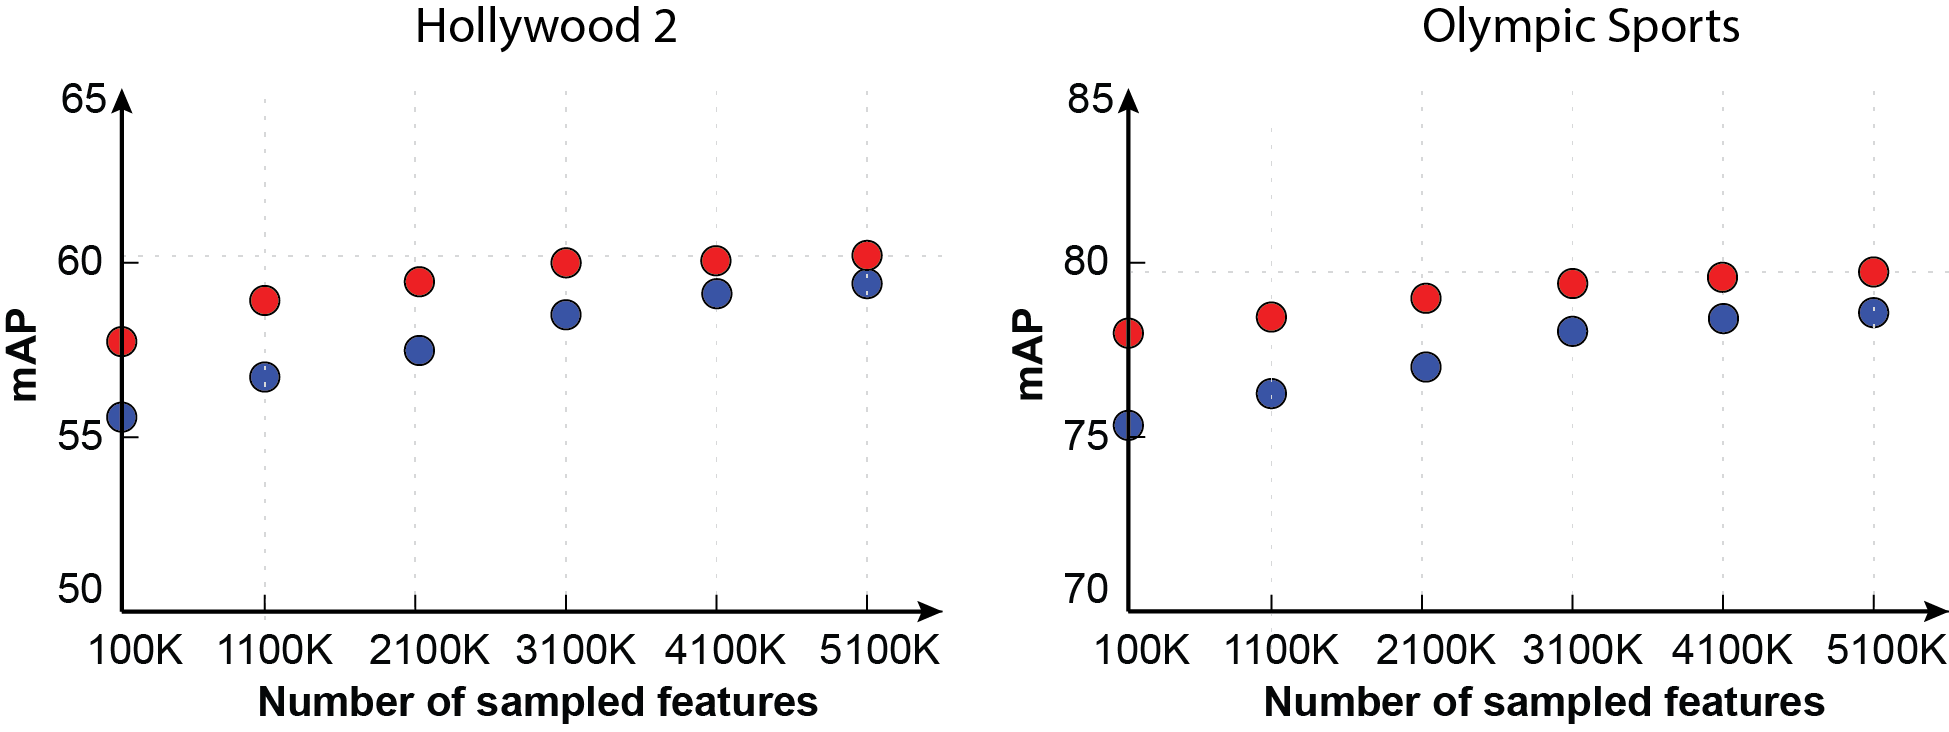
\includegraphics[width=0.98\linewidth]{fig/sampling.png}
\end{center}
\caption{Effect of feature sub-sampling when generating codebook.}
\label{fig:feature_sampling}
\end{figure*}
%%%%%%%%%%%%%%%%%%%%%%%%%%%%%%%%%%%%%%%%%%%%%%%%%%%%%%%%%%%%%%%%

%%%%%%%%%%%%%%% Table: Frameworks comparison %%%%%%%%%%%%%%%%%%%
\begin{table*}[h!]
\caption{Comparison of adopted frameworks for action recognition.}
\begin{center}
{
\begin{tabular}{ l| c c c c c }
\hline
Representation $\downarrow$ & Codebook & Encoding & Normalization & Classifier \\
\hline
Bag of Features & \textit{k}-means & VQ & L2 & MCSVM \\
Fisher vectors & GMM & Fisher vectors & L2+PW+IN & LSVM \\
\hline
\end{tabular}
}
\end{center}
\label{tab:frameworks}
\end{table*}
%%%%%%%%%%%%%%%%%%%%%%%%%%%%%%%%%%%%%%%%%%%%%%%%%%%%%%%%%%%%%%%%

\subsection{Impact of contextual features}
We conduct further experiments to measure the  contribution of our contextual features. Our Baseline corresponds to using only Foreground features for describing actions. Per-descriptor performances are compared to that established baseline. Also, we investigate the effect of combining contextual features with Foreground cues. As well, contextual features performance is evaluated under two action recognition representations \ie Bag of Features and Fisher vectors. Below, we present an analysis of obtained results.\\\\
\textbf{Representation}. As suggested in recent works \cite{perronnin2010, wang2013, xwang2013} Fisher vectors provides a boosted performance compared to traditional Bag of Feature representations. We found in our experiments that Fisher vectors also boost our contextual descriptors performance, as presented in Table \ref{tab:features}. However, we note that using Fisher vectors is less important with our CamMotion descriptor due to its low dimensionality. Even so, Fisher vectors are used for following analysis.\\\\
\textbf{Foreground-background}. As described in Section \ref{scene}, we perform a weak separation between background and foreground feature points. We measure the effect on performance of this separation in our contextual features. We note that this type of weak segmentation provides a significant boost in performance, as observed in Table \ref{tab:segmentation}. When feature points are localized on the background, SIFT features focuses on the scene appearance avoiding information of actors and foreground objects. The gain over computing SIFT over all features points is as follow: +0.3\% for HMDB51, +4.2\% for Hollywood2, +5.2\% for Olympics and +3.9\% for UCF50. The same behavior is observed with our CamMotion descriptor. Performance is boosted in all datasets when Fundamental Matrix is computed based on background tracks.\\\\
\textbf{Context appearance}. While by itself SIFT achieves a discrete performance, it produces notable improvements when combined with foreground descriptors. As Table \ref{tab:features} reports, performance is significantly improved over all datasets. Interestingly, we note that SIFT descriptor produces higher improvements in HMDB51 and UCF50 \ie +2.7\% and +2.4\% respectively.\\\\
\textbf{Camera motion}. Experiment results evidences that action recognition is noticeably improved when a global motion is incorporated to Foreground features. Our CamMotion provides slightly lower contributions in performance than the SIFT descriptor. We observe a significantly contribution over all datasets except on HMDB51 where recognition performance decrease. We attribute this negative effect to that HMDB51 presents several videos containing a shaking camera motion over all classes. This unable our CamMotion to capture discriminative cues over action categories. 

%%%%%%%%%%%%% Table: Effect of selected points %%%%%%%%%%%%%
\begin{table*}
\caption{Effect of separating background feature points on contextual features. Experimental results consistently show that contextual features are better captured on background regions. As observed, SIFT and CamMotion descriptors tend to be more 
discriminative when they are extracted from non-foreground feature points.}
\begin{center}
{
\begin{tabular}{|c|c c|c c c c|}
\hline
& \multicolumn{2}{|c|}{Feature points} & \multicolumn{4}{|c|}{Datasets} \\
Feature $\downarrow$ & Foreground & Background & HMDB51 & Hollywood2 & Olympics & UCF50 \\
\hline
SIFT & \checkmark & & 19.5\% & 22.1\% & 33.5\% & 44.7\% \\
SIFT & & \checkmark & \textbf{20.1\%} & \textbf{28.5\%} & \textbf{39.6\%} & \textbf{49.8\%} \\
SIFT & \checkmark & \checkmark & 19.8\% & 24.3\% & 34.4\% & 45.9\% \\
\hline
CamMotion & \checkmark & & 9.7\% & 14.9\% & 19.5\% & 13.7\% \\
CamMotion & & \checkmark & \textbf{14.1\%} & \textbf{22.1\%} & \textbf{27.2\%} & \textbf{19.5\%} \\
CamMotion & \checkmark & \checkmark & 12.9\% & 18.7\% & 21.8\% & 17.2\% \\
\hline
\end{tabular}
}
\end{center}
\label{tab:segmentation}
\end{table*}
%%%%%%%%%%%%%%%%%%%%%%%%%%%%%%%%%%%%%%%%%%%%%%%%%%%%%%%%%%%%

%%%%%%%%%%%%%% Table: Feature analysis %%%%%%%%%%%%%%%%%%%%%
\begin{table*}
\caption{Impact of our contextual features in recognition performance. Bag of Features generally performs poor than Fisher vectors. Both SIFT and CamMotion show important improvements in performance when they are combined with foreground descriptors.}
\begin{center}
{
\def\arraystretch{1.11}
\setlength{\tabcolsep}{3.66pt}
\begin{tabular}{ |c c c|c c c c| }
\hline
\multicolumn{3}{|c|}{Features} & \multicolumn{4}{|c|}{Datasets} \\
Foreground & SIFT & CamMotion & HMDB51 & Hollywood2 & Olympics & UCF50 \\
\hline
\multicolumn{7}{|c|}{Framework: Bag of Features} \\
\hline
\checkmark & & & 51.2\% & 60.1\% & 79.8\% & 85.9\% \\
& \checkmark & & 19.5\% & 28.7\% & 36.4\% & 45.7\% \\
& & \checkmark & 13.5\% & 21.8\% & 26.9\% & 19.3\% \\
\checkmark & \checkmark & & 53.8\% & 60.9\% & 81.1\% & 87.2\% \\
\checkmark &  & \checkmark & 50.9\% & 60.4\% & 80.6\% & 86.8\% \\
& \checkmark & \checkmark & 20.7\% & 36.2\% & 43.7\% & 50.3\% \\
\checkmark & \checkmark & \checkmark & 51.7\% & 61.6\% & 81.7\% & 87.6\% \\
\hline
\multicolumn{7}{|c|}{Framework: Fisher vectors} \\
\hline
\checkmark & & & 56.5\% & 62.4\% & 90.4\% & 90.9\% \\
& \checkmark & & 20.1\% & 28.5\% & 39.6\% & 49.8\% \\
& & \checkmark & 14.1\% & 22.1\% & 27.2\% & 19.5\% \\
\checkmark & \checkmark & & \textbf{59.2\%} & \textbf{63.5\%} & \textbf{91.6\%} & \textbf{93.3\%} \\
\checkmark &  & \checkmark & 55.9\% & 62.9\% & 91.3\% & 93.1\% \\
& \checkmark & \checkmark & 22.3\% & 36.5\% & 46.5\% & 54.3\% \\
\checkmark & \checkmark & \checkmark & \textbf{57.9\%} & \textbf{64.1\%} & \textbf{92.5\%} & \textbf{93.8\%} \\
\hline
\end{tabular}
}
\end{center}
\label{tab:features}
\end{table*}
%%%%%%%%%%%%%%%%%%%%%%%%%%%%%%%%%%%%%%%%%%%%%%%%%%%%%%%%%%%%%


\subsection{Comparison with the state of the art}
We set side by side our method with recent methods that address the same application using similar representations, \ie methods that use dense trajectory points to represent video sequences \cite{wang2013, jiang2012, jain2013} in Table \ref{tab:stateofart}. We also present results for our own implementation of \cite{wang2013}, which correspond to our baseline (Foreground). The gain over the recent paper \cite{wang2013}, which reports the best performance in the literature, is as follow: \textbf{+2\%} for HMDB51, \textbf{+1.4\%} for Olympic Sports and \textbf{2.6\%} for UCF50. We also achieve a comparable performance on Hollywood2 dataset with only 0.2\% less in the mAP value. Since Human Detection (HD) is not included in our trajectory extraction stage, a more direct comparison its the non-HD approach of Wang \etal \cite{wang2013}. In that case, our method outperforms their improved trajectories in \textbf{3.3\%} for HMDB51, \textbf{1.1\%} for Hollywood2, \textbf{2.3\%} for Olympic Sports and \textbf{3.3\%} for UCF50.

%%%%%%%%%%%%%% Table: State-of-the-art %%%%%%%%%%%%%%%%%%%%%%
\begin{table*}
\caption{Comparison with the state-of-the-art on challenging datasets. Our method improves reported results in the state-of-the-art for three different datasets, HMDB51, Olympic Sports and UCF50 and obtains competitive peformance in Hollywod2.}
\begin{center}
{
\begin{tabular}{ |l| c c c c| }
\hline
Approach $\downarrow$ & HMDB51 & Hollywood2 & Olympics & UCF50 \\
\hline
Jiang \etal \cite{jiang2012} & 40.7\% & 59.5\% & 80.6 & - \\
Jain \etal \cite{jain2013} & 52.1\% & 62.5\% & 83.2 & - \\
Wang \etal \cite{wang2013} non-HD & 55.9\% & 63.0\% & 90.2\% & 90.5\% \\
Wang \etal \cite{wang2013} HD & 57.2\% & \textbf{64.3\%} & 91.1\% & 91.2\% \\
\hline
\multicolumn{5}{|c|}{\textit{Our methods with Fisher vectors}} \\
\hline
Baseline (Foreground) & 56.5\% & 62.4\% & 90.4\% & 90.9\% \\
Foreground + SIFT & \textbf{59.2\%} & 63.5\% & \textbf{91.6\%} & \textbf{93.3\%} \\
Foreground + SIFT + CamMotion  & \textbf{57.9\%} & \textbf{64.1\%} & \textbf{92.5\%} & \textbf{93.8\%} \\
\hline
\end{tabular}
}
\end{center}
\label{tab:stateofart}
\end{table*}
%%%%%%%%%%%%%%%%%%%%%%%%%%%%%%%%%%%%%%%%%%%%%%%%%%%%%%%%%%%%%

\section{Conclusion}
\label{conclusion}

In this paper, we describe the use of camera movement and surrounding scene appearance as cues for action recognition.
Our method is the first to incorporate information about global camera motion as a feature for recognition,
which is shown experimentally to enhance recognition performance in multiple benchmarks. We have also
revisited the use of scene appearance as a feature for action recognition. We show that even a weak foreground/background
segmentation can provide more reliable features related to the surrounding scene compared to the previous
standard practice of using features from the entire frame. We highlight that the use of our camera motion and scene appearance
features in combination with standard motion features that focus on the foreground regions
can lead to state-of-the-art performances when coupled with the simplest classifiers
and encodings used in the current literature.
We expect that more sophisticated modeling frameworks would also be able to leverage our proposed feature extraction
process to further improve the current action recognition performance.

%here would be your acknowledgement (if any) in the final accepted paper

%=============================================================
\bibliographystyle{splncs}
\bibliography{egbib}

%this would normally be the end of your paper, but you may also have an appendix
%within the given limit of number of pages
\end{document}
